\chapter{Wstęp}
\label{chapter-1}

\begin{comment}
Praca dyplomowa przedstawia proces projektowania, programowania oraz budowy modularnego 
urządzenia, którego zadaniem jest testowanie przetwornic napięciowych DC/DC. Przedstawiono 
w niej kolejno projekt elektroniki (rozdział \ref{chapter-2}), przeanalizowano fragmenty kodu źródłowego zastosowanych 
mikrokontrolerów (rozdział \ref{chapter-3}) oraz projekt części mechanicznych (rozdział \ref{chapter-4}).

\section{Cel pracy}
Celem pracy inżynierskiej jest stworzenie urządzenia pozwalającego na szybkie badanie działania 
przetwornic napięciowych DC. 

Przetwornice takie są to urządzenia elektroniczne pozwalające na zmianę wartości 
napięcia wyjściowego w stosunku do napięcia na ich wejściu. Z tego powodu można się również 
spotkać z określeniem "transformatory DC". Wśród nich wyróżnić możemy przetwornice obniżające napięcia (buck),
podwyższające napięcie (boost), pozwalające na podwyższanie oraz obniżanie napięcia (buck-boost) oraz odwracające napięcie (inverting).
Poza klasycznymi topologiami, spotkać się można z przetwornicami typu SEPIC, bądź Ćuk, a także wieloma innymi.

Jeśli chcemy przeanalizować działanie danego układu przetwornicy napięciowej, możemy wziąć pod uwagę jej:
\begin{itemize}
    \item Zakres napięć wejściowych - minimalne oraz maksymalne napięcie wejściowe dla któego przetwornica utrzymuje zadane napięcie wyjśćiowe
    \item Regulacja napięcia wyjściowego - zakres zmian napięcia wyjściowego w pełnym zakresie napięć zasilających i dopuszczalnych prądów obciążenia
    \item Sprawność - stosunek mocy wyjściowej do mocy wejściowej, określający jednocześnie ilość mocy wydzielanej przez samą przetwornicę
    \item Poziom szumów wyjściowych - podawany zazwyczaj jako $V_{RMS}$ oraz $V_{peak-peak}$
\end{itemize}

Przetwornice napięciowe wykorzystywane są obecnie w znaczącej większości urządzeń elektronicznych. Są one elementem niezbędnym do zapewnienia ich poprawnej pracy, 
w związku z czym należy dołożyć szczególnych starań by zapewnić ich bezproblemowe działanie we wszelkich możliwych warunkach. 
W tym celu, jak każde inne urządzenie, należy zaprojektowany układ poddać stosownym testom, które to mają na celu potwierdzenie
osiągnięcia przez nas założonych parametrów pracy układu.

Urządzenie, którego zadaniem ma być pomiar parametrów przetwonic DC/DC, ma więc umożliwić pomiar części spośród wymienionych wyżej parametrów.
W szczególności sprawności oraz zakresu napięć wejściowych. Podczas ręcznego wykonywania takich pomiarów, pomiar sprawności wykonuje się zwykle
dla zadanego napięcia wyjściowego, zmieniając jedynie obciążenie wejściowe. Często dla projektanta ważne jest poznanie sprawności układu
w zależności również od napięcia wejściowego, jak również zbadanie skrajnych wartości napięć wejściowych i prądu obciążenia, dla których 
przetwornica wykazuje się stabilną pracą, zapewniając dalszą regulację napięcia wyjściowego. Wykonywanie tego typu pomiarów jest jednak niezwykle 
uciążliwe z uwagi na konieczność zmiany co najmniej dwóch parametrów jednocześnie. Generuje to olbrzymią ilość danych, a pomiary nierzadko muszą zostać
powtórzone bo wprowadzeniu koniecznych zmian do projektu. 

Z tego też powodu, jednym z głównych celi tej pracy jest przynajmniej częściowa automatyzacja procesu testowania i ułatwienie projektantowi
analizowanie zebranych danych.
\end{comment}

W rozdziale 2 opisano klasyfikację i budowy różnych rodzajów przetwornic DC-DC.

\section{Wstęp teoretyczny - przetwornice napięciowe DC}

Przetwornice napięciowe DC/DC (ang. \textit{DC/DC Converter}), nazywane również przekształtnikami napięcia, bądź konwerterami mocy 
\cite{przetworncieNapieciowe}, to układy umożliwiające zmianę napięć i prądów w celu poprawnego zasilania 
innych urządzeń elektronicznych / elektrycznych. Zadanie, polegające na dostarczeniu do obciążenia wymaganej wartości napięcia, realizować można na kilka sposobów, w zależności od dostępnych dla projektanta źródeł mocy (napięcia lub prądu), a także oczekiwanej sprawności kompletnego rozwiązania.

Rozważając wyłącznie zmianę napięcia DC na DC, przy założeniu, że napięcie dostarczane do obciążenia ma być mniejsze niż wejściowe, zastosować można proste dzielniki rezystancyjne, bądź regulatory liniowe.
Główną wadą takiego rozwiązanie jest jednak niska sprawność, czyli stosunek mocy dostarczanej do obciążenia, do mocy pobieranej przez układ zasilacza, zgodnie ze wzorem \ref{eq:1}.

\begin{equation}
    \label{eq:1}
    \eta = \frac{P_{load}}{P_{in}}
\end{equation}

Jeśli więc potrzebne jest podwyższenie napięcia, odwrócenie jego polaryzacji, bądź konieczne jest zwiększenie sprawności zasilacza, najbardziej optymalnym rozwiązaniem okazuje się przetwornica impulsowa.
Przetwornice impulsowe, inaczej zasilacze impulsowe (ang. SMPS - \textit{Switch Mode Power Supply}) \cite{zasilaczeImpulsowe}, umożliwiają podwyższanie, obniżanie i odwracanie napięć wejściowych oraz cechują się wysoką, w porównaniu do innych rozwiązań, sprawnością.

Wyróżnić należy w tym miejscu trzy podstawowe typy przetwornic impulsowych DC/DC, czyli przekształcających napięcia stałe:

\begin{itemize}
    \item buck - przetwornica obniżająca napięcie,
    \item boost - przetwornica podwyższająca napięcie,
    \item buck-boost - przetwornica umożliwiająca zarówno obniżanie jak i podwyższanie napięcia wejściowego.
\end{itemize}

Na rysunku \ref{fig:przetwornice} przedstawiono przykładowe schematy układów realizujących te trzy typy przetwornic napięciowych.

\begin{figure}[h!]
    \begin{center}
        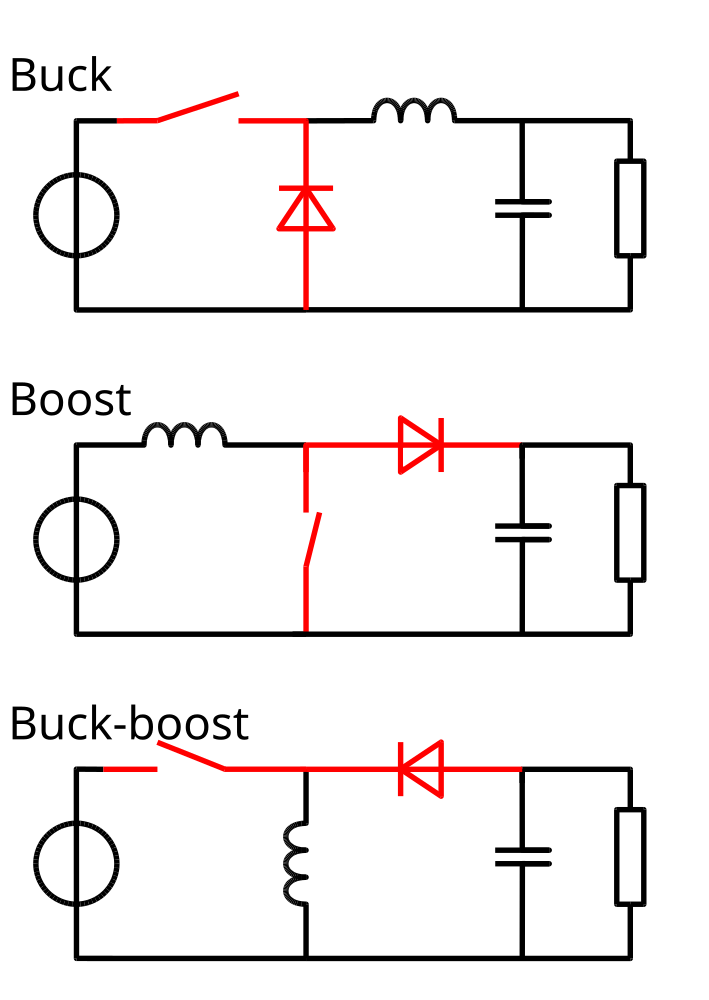
\includegraphics[width = 10cm]{images/przetworniceDC.png}
        \caption{Przetwornice typu buck, boost oraz buck-boost.}
        \label{fig:przetwornice}
    \end{center}
\end{figure}

Istnieją także inne implementacje przetwornic napięciowych, takie jak np.: Ćuk, SEPIC. Ze względu m.in. na ich skomplikowaną konstrukcję (np. stosowanie kondensatora szeregowego), są one dużo mniej popularne od powyżej przedstawionych.
W przypadku konwertera typu buck-boost, należy zauważyć, iż odwraca on napięcie wejściowe, w związku z czym w niektórych przypadkach stosuje się zamiast tego szeregowe połączenie układów buck oraz boost, w celu zachowania polaryzacji napięcia względem wspólnej masy.




\section{Prezentacja problemu}

Przetwornice napięciowe znalazły zastosowanie w znacznej większości urządzeń elektronicznych. Są one stosowane w komputerach, telefonach, zegarkach, urządzeniach medycznych, automatyce, a obecnie nawet w wielu urządzeniach laboratoryjnych i profesjonalnym sprzęcie pomiarowym.
Na stosowanie w tak szerokim zakresie aplikacji, niekiedy bardzo wymagających, pozwolił rozwój półprzewodników, w tym powstanie układów GaN, tranzystorów HEMT i innych, a także integracja niezbędnych elementów przełączających w niewielkich układach scalonych. 
Do dziś, największym problemem pozostają elementy magnetyczne (cewki) oraz kondensatory. W związku z tym, współczesne zasilacze impulsowe pracują z coraz to większymi częstotliwościami przełączania, a co za tym idzie, rosną wymagania co do ich elementów składowych.

Projektanci mają więc do wyboru wiele układów scalonych, elementów przełączających, jak i pasywnych, które należy dobrać odpowiednio do danego zastosowania.
W tym celu, należy znać podstawowe parametry przetwornicy, takie jak:

\begin{itemize}
    \item zakres napięć wejściowych - minimalne oraz maksymalne napięcie wejściowe, dla którego przetwornica utrzymuje zadane napięcie wyjściowe,
    \item regulacja napięcia wyjściowego - zakres zmian napięcia wyjściowego w pełnym zakresie napięć zasilających i dopuszczalnych prądów obciążenia,
    \item sprawność - stosunek mocy wyjściowej do mocy wejściowej, określający jednocześnie ilość mocy wydzielanej przez samą przetwornicę, zgodnie z \ref{eq:1},
    \item poziom szumów wyjściowych - podawany zazwyczaj jako $V_{RMS}$ oraz $V_{peak-peak}$,
    \item fizyczne wymiary układu - ograniczone m.in. pobieraną mocą i częstotliwością przełączania.
\end{itemize}

W zastosowaniach precyzyjnych, takich jak urządzenia pomiarowe, niewątpliwie 
najważniejszą cechą będzie poziom szumów. Jeśli jednak urządzenie zasilane jest 
bateryjnie i wymaga się od niego długiego czasu pracy, konieczne okaże się 
zoptymalizowanie projektu pod kątem sprawności. Niestety, nie jest się  w stanie 
poprawić każdego parametru z osobna, nie wpływając na pozostałe. 

Dzięki rozwojowi technologii, konstruktor może obecnie symulować działanie zasilacza, korzystając z 
oprogramowania takiego jak np. SPICE \cite{spice}. Pozwala to na przewidywanie zachowania 
projektowanego układu jeszcze przed jego skonstruowaniem. Niestety, na parametry 
finalnego produktu wpłynąć mogą elementy pasożytnicze i rozbieżność parametrów modeli 
elementów, które są stosowane. Konieczna jest więc weryfikacja fizycznego układu i jego
pomiary.

Do najpopularniejszych pomiarów należą:

\begin{comment}
W zastosowaniach precyzyjnych, takich jak urządzenia pomiarowe, niewątpliwie najważniejszą cechą będzie poziom szumów. Jeśli jednak nasze urządzenie zasilane jest bateryjnie i wymagamy od niego długiego czasu pracy, konieczne okaże się zoptymalizowanie projektu pod kątem sprawności.
Niestety, nie jesteśmy w  stanie poprawić każdego parametru z osobna, nie wpływając na pozostałe.

Dzięki rozwojowi technologii, jesteśmy obecnie w stanie symulować działanie zasilacza, korzystając z oprogramowania takiego jak np. SPICE \cite{spice}.
Pozwala to na przewidywanie zachowania projektowanego układu jeszcze przed jego skonstruowaniem. Niestety, na parametry finalnego produktu wpłynąć mogą elementy pasożytnicze i rozbieżność parametrów modeli elementów, które stosujemy.
Konieczna jest więc weryfikacja fizycznego układu i jego pomiary. 

Do najpopularniejszych pomiarów należą: 
\end{comment}

\begin{itemize}
    \item pomiar szumów wyjściowych - wykonywany zwykle pod obciążeniem, za pomocą oscyloskopu, bądź analizatora widma,
    \item pomiar regulacji napięcia wyjściowego - wykonywany przy pomocy woltomierza pod obciążeniem,
    \item pomiar sprawności - wymagane jest tu zmierzenie poziomu mocy wejściowej i wyjściowej dla danego obciążenia. 
\end{itemize}

Zdecydowanie najbardziej czasochłonnym z powyższych staje się pomiar sprawności. Jeśli bowiem chcemy zbadać sprawność przetwornicy w szerokim zakresie napięć wejściowych, czy też prądów obciążenia, 
dokonujemy wielu pomiarów, których wynikiem są np. przedstawione tu wykresy \ref{fig:przykladowaSprawnosc}.

\begin{figure}[h!]
    \begin{center}
        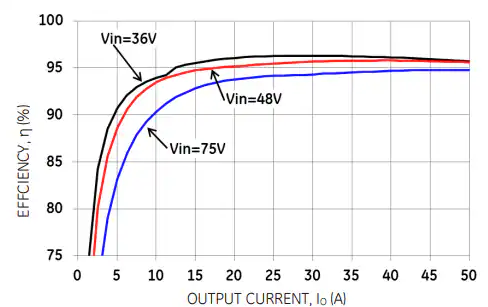
\includegraphics[width = 10cm]{images/przykladowaSprawnosc.png}
        \caption{Przykładowy wykres sprawności przetwornicy w zależności od napięcia wejściowego i prądu obciążenia, źródło: \cite{przetwornicaOmniON}.}
        \label{fig:przykladowaSprawnosc}
    \end{center}
\end{figure}

Do wykonania takiego pomiaru, potrzebne są zazwyczaj:

\begin{itemize}
    \item zasilacz regulowany - zasilający mierzoną przetwornicę,
    \item obciążenie aktywne - pozwalające na zmianę pobieranego z przetwornicy prądu,
    \item dwa woltomierze - do pomiaru napięcia wejściowego i wyjściowego,
    \item dwa amperomierze - do pomiaru prądów wejściowego i wyjściowego.
\end{itemize}

Zakładając, że woltomierze i amperomierze (pomiar mocy) są zintegrowane w układy zasilacza i obciążenia aktywnego, potrzebne są jedynie te dwa urządzenia.
Niestety, często konieczne jest ręczne zapisywanie wyników każdego pomiaru i ponowna zmiana ustawień obu urządzeń, a następnie obróbka otrzymanych danych.

Rozwiązania tego problemu, które mogą skrócić czas i usprawnić proces charakteryzacji przetwornicy, przedstawione zostaną w rozdziale \ref{chapter-2} 
wraz z projektowanym urządzeniem, które integruje niezbędne do wykonania pomiarów elementy.


